%%%%%%%%%%%%%%%%%%%%%%%%%%%%%%%%%%%%%%%%%
% University Project Report Page 
% LaTeX Template
% Version 1.0 (27/12/12)
%
% This template has been downloaded from:
% http://www.LaTeXTemplates.com
%
% Original author:
% WikiBooks (http://en.wikibooks.org/wiki/LaTeX/Title_Creation)
%
% License:
% CC BY-NC-SA 3.0 (http://creativecommons.org/licenses/by-nc-sa/3.0/)
% 
% Instructions for using this template:
% This title page is capable of being compiled as is. This is not useful for 
% including it in another document. To do this, you have two options: 
%
% 1) Copy/paste everything between \begin{document} and \end{document} 
% starting at \begin{titlepage} and paste this into another LaTeX file where you 
% want your title page.
% OR
% 2) Remove everything outside the \begin{titlepage} and \end{titlepage} and 
% move this file to the same directory as the LaTeX file you wish to add it to. 
% Then add %%%%%%%%%%%%%%%%%%%%%%%%%%%%%%%%%%%%%%%%%
% University Project Report Page 
% LaTeX Template
% Version 1.0 (27/12/12)
%
% This template has been downloaded from:
% http://www.LaTeXTemplates.com
%
% Original author:
% WikiBooks (http://en.wikibooks.org/wiki/LaTeX/Title_Creation)
%
% License:
% CC BY-NC-SA 3.0 (http://creativecommons.org/licenses/by-nc-sa/3.0/)
% 
% Instructions for using this template:
% This title page is capable of being compiled as is. This is not useful for 
% including it in another document. To do this, you have two options: 
%
% 1) Copy/paste everything between \begin{document} and \end{document} 
% starting at \begin{titlepage} and paste this into another LaTeX file where you 
% want your title page.
% OR
% 2) Remove everything outside the \begin{titlepage} and \end{titlepage} and 
% move this file to the same directory as the LaTeX file you wish to add it to. 
% Then add %%%%%%%%%%%%%%%%%%%%%%%%%%%%%%%%%%%%%%%%%
% University Project Report Page 
% LaTeX Template
% Version 1.0 (27/12/12)
%
% This template has been downloaded from:
% http://www.LaTeXTemplates.com
%
% Original author:
% WikiBooks (http://en.wikibooks.org/wiki/LaTeX/Title_Creation)
%
% License:
% CC BY-NC-SA 3.0 (http://creativecommons.org/licenses/by-nc-sa/3.0/)
% 
% Instructions for using this template:
% This title page is capable of being compiled as is. This is not useful for 
% including it in another document. To do this, you have two options: 
%
% 1) Copy/paste everything between \begin{document} and \end{document} 
% starting at \begin{titlepage} and paste this into another LaTeX file where you 
% want your title page.
% OR
% 2) Remove everything outside the \begin{titlepage} and \end{titlepage} and 
% move this file to the same directory as the LaTeX file you wish to add it to. 
% Then add %%%%%%%%%%%%%%%%%%%%%%%%%%%%%%%%%%%%%%%%%
% University Project Report Page 
% LaTeX Template
% Version 1.0 (27/12/12)
%
% This template has been downloaded from:
% http://www.LaTeXTemplates.com
%
% Original author:
% WikiBooks (http://en.wikibooks.org/wiki/LaTeX/Title_Creation)
%
% License:
% CC BY-NC-SA 3.0 (http://creativecommons.org/licenses/by-nc-sa/3.0/)
% 
% Instructions for using this template:
% This title page is capable of being compiled as is. This is not useful for 
% including it in another document. To do this, you have two options: 
%
% 1) Copy/paste everything between \begin{document} and \end{document} 
% starting at \begin{titlepage} and paste this into another LaTeX file where you 
% want your title page.
% OR
% 2) Remove everything outside the \begin{titlepage} and \end{titlepage} and 
% move this file to the same directory as the LaTeX file you wish to add it to. 
% Then add \input{./title_page_1.tex} to your LaTeX file where you want your
% title page.
%
%%%%%%%%%%%%%%%%%%%%%%%%%%%%%%%%%%%%%%%%%
%\title{Title page with logo}
%----------------------------------------------------------------------------------------
%	PACKAGES AND OTHER DOCUMENT CONFIGURATIONS
%----------------------------------------------------------------------------------------

\documentclass[12pt]{article}
\usepackage[english]{babel}
\usepackage[utf8x]{inputenc}
\usepackage{amsmath}
\usepackage{graphicx}
\usepackage[colorinlistoftodos]{todonotes}

\begin{document}

\begin{titlepage}

\newcommand{\HRule}{\rule{\linewidth}{0.5mm}} % Defines a new command for the horizontal lines, change thickness here

\center % Center everything on the page
 
%----------------------------------------------------------------------------------------
%	HEADING SECTIONS
%----------------------------------------------------------------------------------------

\textsc{\LARGE University of California, Santa Barbara}\\[1cm] % Name of your university/college
\textsc{\Large Project Report}\\[0.5cm] % Major heading such as course name

%----------------------------------------------------------------------------------------
%	TITLE SECTION
%----------------------------------------------------------------------------------------

\HRule \\[0.4cm]
{ \huge \bfseries Image Captioning}\\[0.1cm] % Title of your document
\HRule \\[1cm]
 
%----------------------------------------------------------------------------------------
%	AUTHOR SECTION
%----------------------------------------------------------------------------------------

\begin{minipage}{0.4\textwidth}
\begin{flushleft} \large
\emph{Author:}\\
Nikhil \textsc{S M} \\
Rahul \textsc{V} % Your name
\end{flushleft}
\end{minipage}
~
\begin{minipage}{0.4\textwidth}
\begin{flushright} \large
\emph{Supervisor:} \\
Prof Y F \textsc{Wang} % Supervisor's Name
\end{flushright}
\end{minipage}\\[2cm]

% If you don't want a supervisor, uncomment the two lines below and remove the section above
%\Large \emph{Author:}\\
%John \textsc{Smith}\\[3cm] % Your name

%----------------------------------------------------------------------------------------
%	DATE SECTION
%----------------------------------------------------------------------------------------

{\large \today}\\[1cm] % Date, change the \today to a set date if you want to be precise

%----------------------------------------------------------------------------------------
%	LOGO SECTION
%----------------------------------------------------------------------------------------


\includegraphics{assets/ucsb-logo.png}\\[1cm] % Include a department/university logo - this will require the graphicx package
 
%----------------------------------------------------------------------------------------
\vfill % Fill the rest of the page with whitespace
\end{titlepage}

%\begin{abstract}
%\end{abstract}

%----------------------------------------------------------------------------------------
\section{Objective}
Understand the Image Captioning problem in Computer vision and Natural language processing. Demonstrate components, process, training ( with batching, validation) and estimate performance (e.g., error rate vs. run time and iterations, resource usage statistics)
% section ends 

%----------------------------------------------------------------------------------------
\section{Introduction}
Automatically describing the contents of an image is a fundamental problem in computer vision and natural language processing. In this project we look at a generative model based on a deep recurrent architecture. The model is trained to maximize the likelihood of the target description sentence given the training image. Experiments on COCO image/text datasets show the accuracy of the model and the fluency of the language it learns solely from image descriptions.

This project based its implementation on the method described in the CVPR2015 paper "Show and Tell: A Neural Image Caption Generator". 
% section ends 

%----------------------------------------------------------------------------------------
\section{Model}
Model is based end-to-end on a neural network consisting of a vision CNN followed by a language generating RNN. The author's describe this model as Neural Image Caption or NIC.
% Include a shownntell figure here:
\begin{figure}[ht!]
\centering
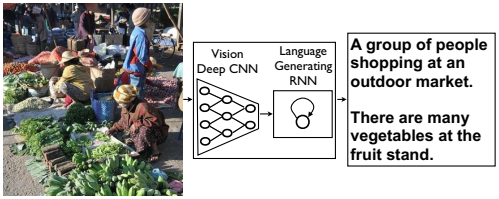
\includegraphics[width=0.8\textwidth]{assets/shownntell.png}
\caption{\label{fig:shownntell}NIC model (vision CNN followed by language generating RNN)}
\end{figure}

An “encoder” CNN reads the input images by embedding it to a fixed-length vector and transforms it into a rich fixed-length vector representation, which is pre-trained for an image classification task and using the last hidden layer as the initial hidden state of a “decoder” RNN that generates the target sentence. The RNN model uses a Long-Short Term Memory (LSTM) net, which has shown state-of-the art performance on sequence tasks such as translation.

% Include a model figure here:
\begin{figure}[ht!]
\centering
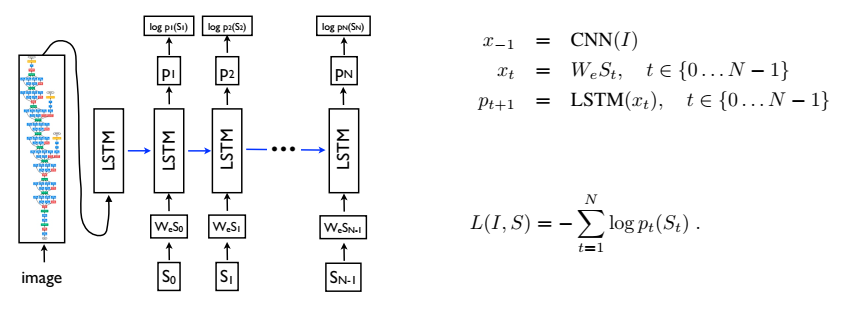
\includegraphics[width=1\textwidth]{assets/model.png}
\caption{\label{fig:model}LSTM model combined with a CNN image embedder. L(I,S) is the loss function with each word as a one-hot vector S\textsubscript{t}}.
\end{figure}

Both the image and the words are mapped to the same space, the image by using a vision CNN, the words by using word embedding W\textsubscript{e}. Inference is done by BeamSearch, keeping k best sentences up to time t as candidates to generate sentences of size t+1 and taking the resulting best.
% section ends 

%----------------------------------------------------------------------------------------
\section{Results}
\label{sec:results}

\subsection{Training}
The MS COCO dataset consists of JPEG images and text captions for each image.



Here is a brief on the training data configuration
% Describe the dataset
\begin{table}[ht!]
\centering
  \begin{tabular}{l|l|l|l}
    Dataset & training & valid & test  \\\hline
    MSCOCO & 82783 & 40504 & 40775\\
  \end{tabular}
\caption{\label{tab:dataset} MSCOCO Dataset}
\label{tab:dataset}
\end{table}

\begin{description}
  \item[$\bullet$ ] Initialized weights of CNN component to a pre-trained model (ImageNet).
  \item[$\bullet$ ] Preprocessing of MS-Coco Data set
  	\begin{description}
    	\item[$\cdot$ ] Creating a correspondence between image and the caption.
    \end{description}
  \item[$\bullet$ ] Creating a Word Embedding Matrix.
  \item[$\bullet$ ] Cross Entropy as Loss function
  \item[$\bullet$ ] Adam Optimizer with initial learning rate of 0.0001
  \item[$\bullet$ ] Training: 
    \begin{description}
      	\item[$\cdot$ ] Data Set : MS COCO as per Table~\ref{tab:dataset}
      	\item[$\cdot$ ] All RNN inputs are left padded.
      	\item[$\cdot$ ] Words are Embedded into 512 dimension vector.
      	\item[$\cdot$ ] A Batch size of 32 is used to run for 5 epochs.
      	\item[$\cdot$ ] BLEU Score is used as an evaluation metric.
    \end{description}
  \item[$\cdot$ ] Data Set : MS COCO as per Table~\ref{tab:dataset}
  \item[$\ast$ ]
\end{description}

Lets take a look at the workflow for establishing the training data

Data Description
The COCO data has JPG images with text captions for each image in a JSON file. We use the "image\_id", "image\_file" and "caption" fields from the captions .... 


\todo[inline, color=green!40]{Describe the training parameters measure, accuracies \& convergence}



\subsection{Metrics}
Here are the various metrics for MS COCO dataset. 
\todo{Describe the metrics!}
% Describe the metrics
\begin{table}[h!]
\centering
\begin{tabular}{l|l|l|l|l}
Metric & BLEU-1 & BLEU-2 & BLEU-3 & BLEU-4  \\\hline
Value & 62.9\% & 43.6\% & 29.0\% & 19.3\% \\
\end{tabular}
\caption{\label{tab:metrics}Scores on Dataset --- described in Table~\ref{tab:dataset}.}
\end{table}
% subsection ends 
%----------------

\subsection{Output}
Here are some test outputs generated by the Image captioning system \dots

\subsubsection{Images from the internet }
\begin{figure}[ht!]
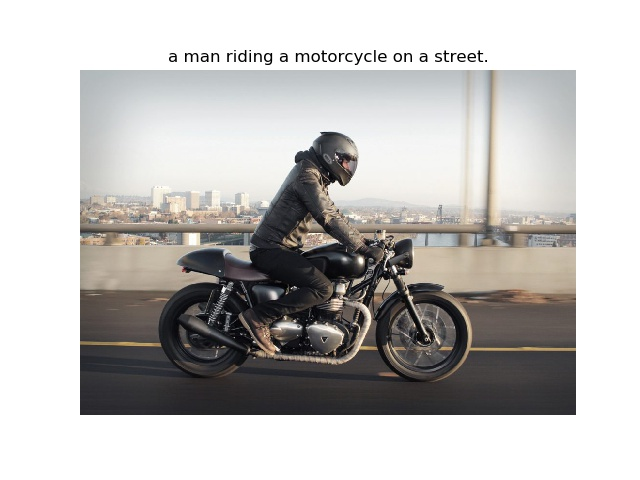
\includegraphics[width=0.75\textwidth]{assets/eg/r2_out.jpg}
\end{figure}
\begin{figure}[ht!]
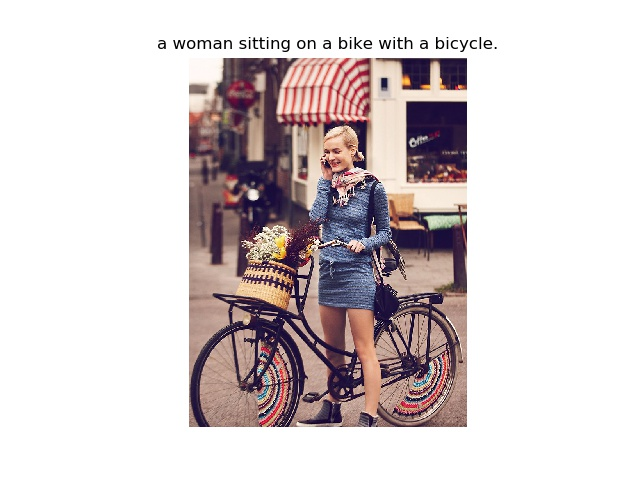
\includegraphics[width=0.75\textwidth]{assets/eg/r3_out.jpg}
\end{figure}
\begin{figure}[ht!]
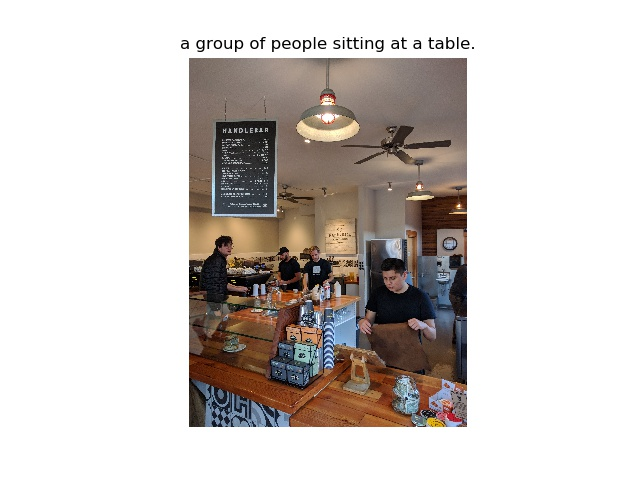
\includegraphics[width=0.75\textwidth]{assets/eg/r4_out.jpg}
\end{figure}

\subsubsection{Images from the Arrowhead common rooms}
\begin{figure}[ht!]
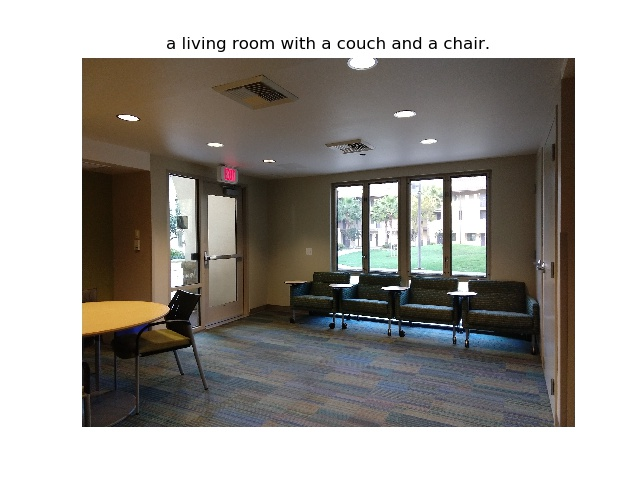
\includegraphics[width=0.75\textwidth]{assets/eg/r5_out.jpg}
\end{figure}
\begin{figure}[ht!]
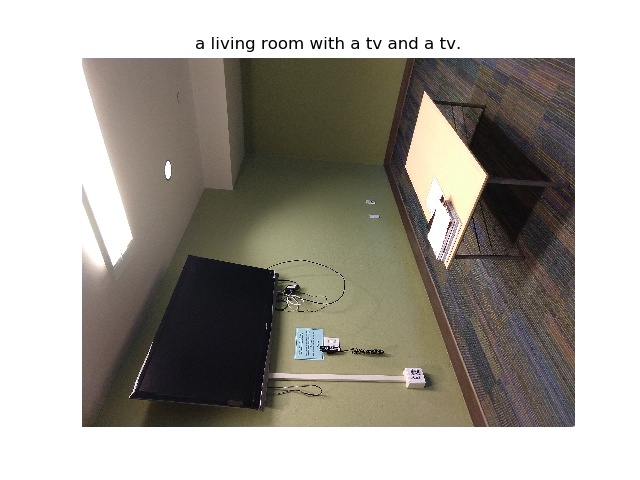
\includegraphics[width=0.75\textwidth]{assets/eg/r6_out.jpg}
\end{figure}
\begin{figure}[ht!]
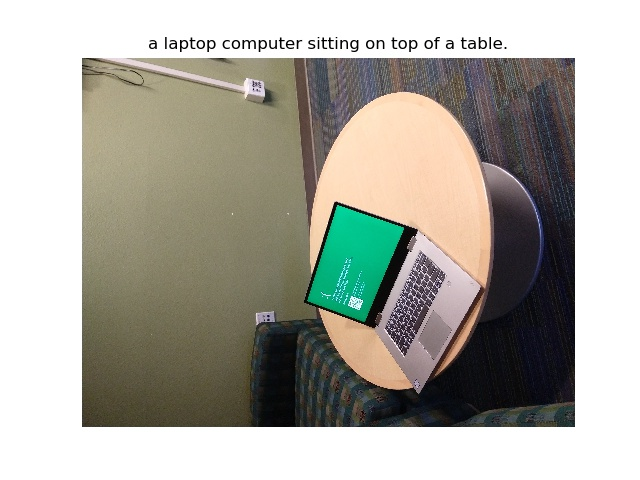
\includegraphics[width=0.75\textwidth]{assets/eg/r7_out.jpg}
\end{figure}
% subsection ends 
%----------------

\subsection{Conclusion}
It is clear from these experiments that, as the size of the available datasets for image description increases, so will the performance of approaches like NIC. However there are many scenarios on which the current model shows errors like the one here.
\begin{figure}[h!]
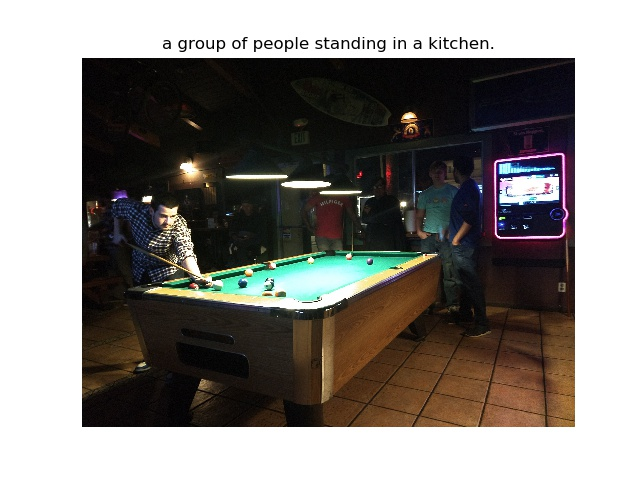
\includegraphics[width=0.75\textwidth]{assets/eg/err1_out.jpg}
\end{figure}
% subsection ends 
%----------------

%----------------------------------------------------------------------------------------

% section ends 
\LaTeX\
\end{document} to your LaTeX file where you want your
% title page.
%
%%%%%%%%%%%%%%%%%%%%%%%%%%%%%%%%%%%%%%%%%
%\title{Title page with logo}
%----------------------------------------------------------------------------------------
%	PACKAGES AND OTHER DOCUMENT CONFIGURATIONS
%----------------------------------------------------------------------------------------

\documentclass[12pt]{article}
\usepackage[english]{babel}
\usepackage[utf8x]{inputenc}
\usepackage{amsmath}
\usepackage{graphicx}
\usepackage[colorinlistoftodos]{todonotes}

\begin{document}

\begin{titlepage}

\newcommand{\HRule}{\rule{\linewidth}{0.5mm}} % Defines a new command for the horizontal lines, change thickness here

\center % Center everything on the page
 
%----------------------------------------------------------------------------------------
%	HEADING SECTIONS
%----------------------------------------------------------------------------------------

\textsc{\LARGE University of California, Santa Barbara}\\[1cm] % Name of your university/college
\textsc{\Large Project Report}\\[0.5cm] % Major heading such as course name

%----------------------------------------------------------------------------------------
%	TITLE SECTION
%----------------------------------------------------------------------------------------

\HRule \\[0.4cm]
{ \huge \bfseries Image Captioning}\\[0.1cm] % Title of your document
\HRule \\[1cm]
 
%----------------------------------------------------------------------------------------
%	AUTHOR SECTION
%----------------------------------------------------------------------------------------

\begin{minipage}{0.4\textwidth}
\begin{flushleft} \large
\emph{Author:}\\
Nikhil \textsc{S M} \\
Rahul \textsc{V} % Your name
\end{flushleft}
\end{minipage}
~
\begin{minipage}{0.4\textwidth}
\begin{flushright} \large
\emph{Supervisor:} \\
Prof Y F \textsc{Wang} % Supervisor's Name
\end{flushright}
\end{minipage}\\[2cm]

% If you don't want a supervisor, uncomment the two lines below and remove the section above
%\Large \emph{Author:}\\
%John \textsc{Smith}\\[3cm] % Your name

%----------------------------------------------------------------------------------------
%	DATE SECTION
%----------------------------------------------------------------------------------------

{\large \today}\\[1cm] % Date, change the \today to a set date if you want to be precise

%----------------------------------------------------------------------------------------
%	LOGO SECTION
%----------------------------------------------------------------------------------------


\includegraphics{assets/ucsb-logo.png}\\[1cm] % Include a department/university logo - this will require the graphicx package
 
%----------------------------------------------------------------------------------------
\vfill % Fill the rest of the page with whitespace
\end{titlepage}

%\begin{abstract}
%\end{abstract}

%----------------------------------------------------------------------------------------
\section{Objective}
Understand the Image Captioning problem in Computer vision and Natural language processing. Demonstrate components, process, training ( with batching, validation) and estimate performance (e.g., error rate vs. run time and iterations, resource usage statistics)
% section ends 

%----------------------------------------------------------------------------------------
\section{Introduction}
Automatically describing the contents of an image is a fundamental problem in computer vision and natural language processing. In this project we look at a generative model based on a deep recurrent architecture. The model is trained to maximize the likelihood of the target description sentence given the training image. Experiments on COCO image/text datasets show the accuracy of the model and the fluency of the language it learns solely from image descriptions.

This project based its implementation on the method described in the CVPR2015 paper "Show and Tell: A Neural Image Caption Generator". 
% section ends 

%----------------------------------------------------------------------------------------
\section{Model}
Model is based end-to-end on a neural network consisting of a vision CNN followed by a language generating RNN. The author's describe this model as Neural Image Caption or NIC.
% Include a shownntell figure here:
\begin{figure}[ht!]
\centering
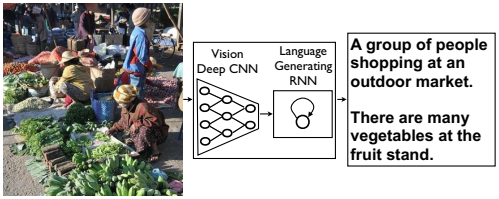
\includegraphics[width=0.8\textwidth]{assets/shownntell.png}
\caption{\label{fig:shownntell}NIC model (vision CNN followed by language generating RNN)}
\end{figure}

An “encoder” CNN reads the input images by embedding it to a fixed-length vector and transforms it into a rich fixed-length vector representation, which is pre-trained for an image classification task and using the last hidden layer as the initial hidden state of a “decoder” RNN that generates the target sentence. The RNN model uses a Long-Short Term Memory (LSTM) net, which has shown state-of-the art performance on sequence tasks such as translation.

% Include a model figure here:
\begin{figure}[ht!]
\centering
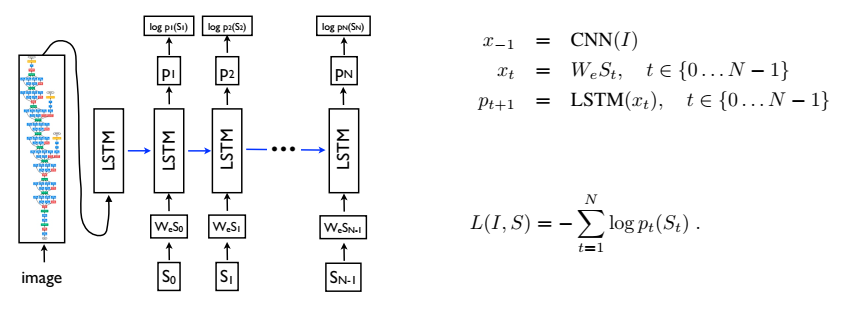
\includegraphics[width=1\textwidth]{assets/model.png}
\caption{\label{fig:model}LSTM model combined with a CNN image embedder. L(I,S) is the loss function with each word as a one-hot vector S\textsubscript{t}}.
\end{figure}

Both the image and the words are mapped to the same space, the image by using a vision CNN, the words by using word embedding W\textsubscript{e}. Inference is done by BeamSearch, keeping k best sentences up to time t as candidates to generate sentences of size t+1 and taking the resulting best.
% section ends 

%----------------------------------------------------------------------------------------
\section{Results}
\label{sec:results}

\subsection{Training}
The MS COCO dataset consists of JPEG images and text captions for each image.



Here is a brief on the training data configuration
% Describe the dataset
\begin{table}[ht!]
\centering
  \begin{tabular}{l|l|l|l}
    Dataset & training & valid & test  \\\hline
    MSCOCO & 82783 & 40504 & 40775\\
  \end{tabular}
\caption{\label{tab:dataset} MSCOCO Dataset}
\label{tab:dataset}
\end{table}

\begin{description}
  \item[$\bullet$ ] Initialized weights of CNN component to a pre-trained model (ImageNet).
  \item[$\bullet$ ] Preprocessing of MS-Coco Data set
  	\begin{description}
    	\item[$\cdot$ ] Creating a correspondence between image and the caption.
    \end{description}
  \item[$\bullet$ ] Creating a Word Embedding Matrix.
  \item[$\bullet$ ] Cross Entropy as Loss function
  \item[$\bullet$ ] Adam Optimizer with initial learning rate of 0.0001
  \item[$\bullet$ ] Training: 
    \begin{description}
      	\item[$\cdot$ ] Data Set : MS COCO as per Table~\ref{tab:dataset}
      	\item[$\cdot$ ] All RNN inputs are left padded.
      	\item[$\cdot$ ] Words are Embedded into 512 dimension vector.
      	\item[$\cdot$ ] A Batch size of 32 is used to run for 5 epochs.
      	\item[$\cdot$ ] BLEU Score is used as an evaluation metric.
    \end{description}
  \item[$\cdot$ ] Data Set : MS COCO as per Table~\ref{tab:dataset}
  \item[$\ast$ ]
\end{description}

Lets take a look at the workflow for establishing the training data

Data Description
The COCO data has JPG images with text captions for each image in a JSON file. We use the "image\_id", "image\_file" and "caption" fields from the captions .... 


\todo[inline, color=green!40]{Describe the training parameters measure, accuracies \& convergence}



\subsection{Metrics}
Here are the various metrics for MS COCO dataset. 
\todo{Describe the metrics!}
% Describe the metrics
\begin{table}[h!]
\centering
\begin{tabular}{l|l|l|l|l}
Metric & BLEU-1 & BLEU-2 & BLEU-3 & BLEU-4  \\\hline
Value & 62.9\% & 43.6\% & 29.0\% & 19.3\% \\
\end{tabular}
\caption{\label{tab:metrics}Scores on Dataset --- described in Table~\ref{tab:dataset}.}
\end{table}
% subsection ends 
%----------------

\subsection{Output}
Here are some test outputs generated by the Image captioning system \dots

\subsubsection{Images from the internet }
\begin{figure}[ht!]
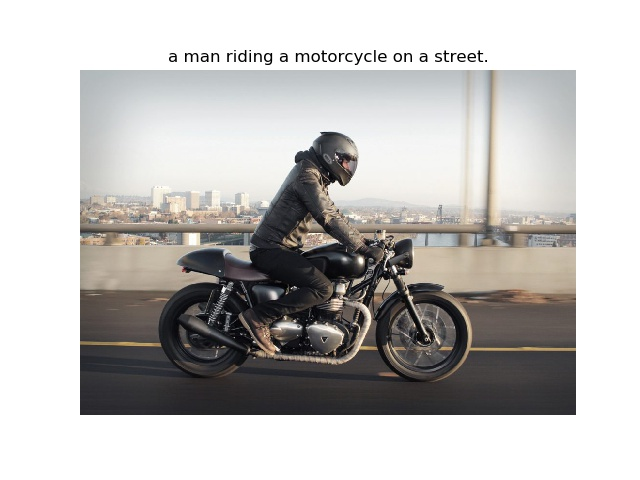
\includegraphics[width=0.75\textwidth]{assets/eg/r2_out.jpg}
\end{figure}
\begin{figure}[ht!]
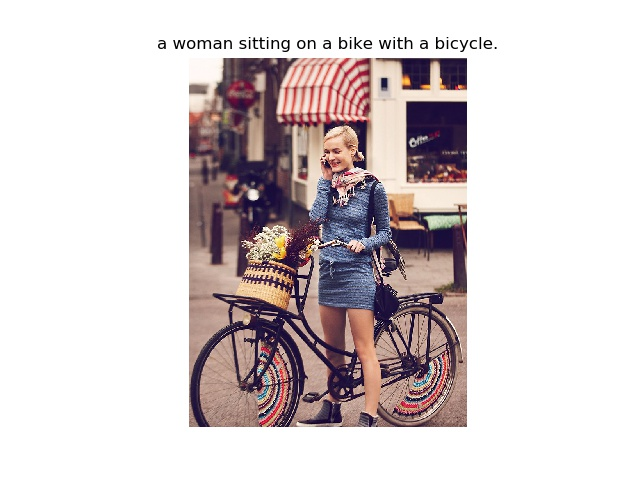
\includegraphics[width=0.75\textwidth]{assets/eg/r3_out.jpg}
\end{figure}
\begin{figure}[ht!]
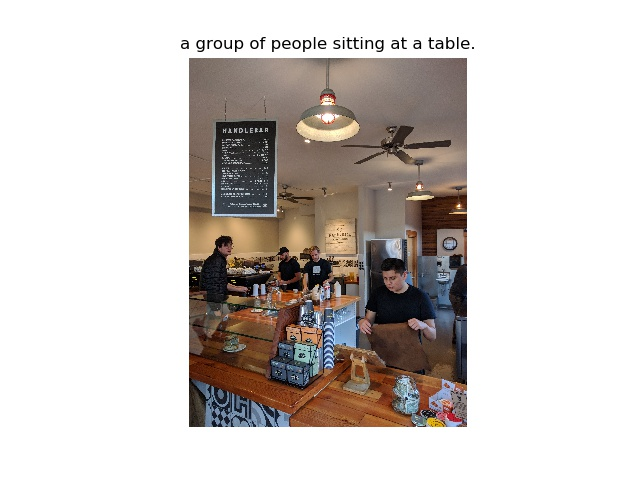
\includegraphics[width=0.75\textwidth]{assets/eg/r4_out.jpg}
\end{figure}

\subsubsection{Images from the Arrowhead common rooms}
\begin{figure}[ht!]
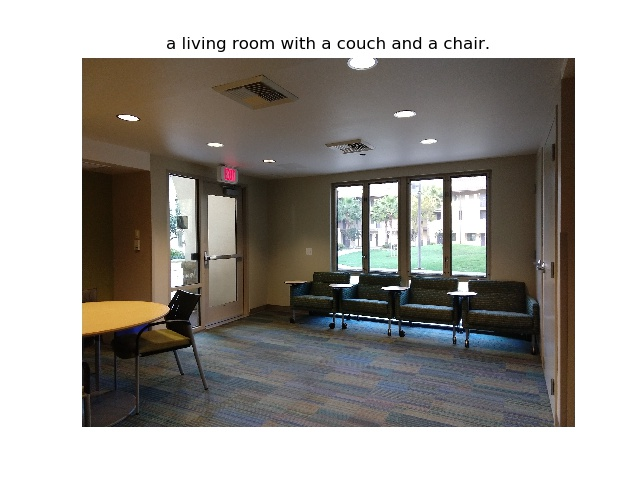
\includegraphics[width=0.75\textwidth]{assets/eg/r5_out.jpg}
\end{figure}
\begin{figure}[ht!]
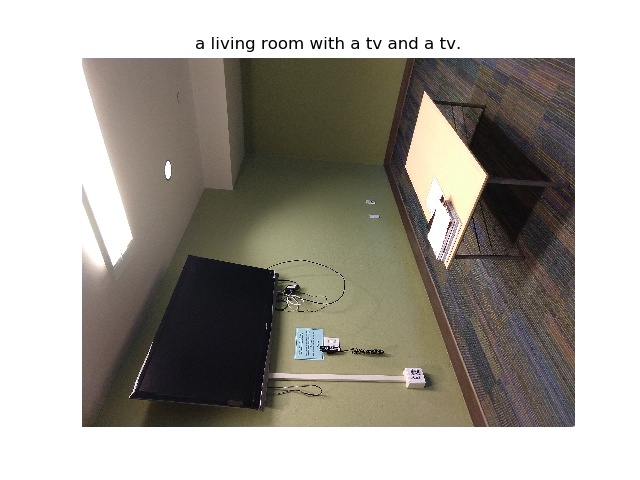
\includegraphics[width=0.75\textwidth]{assets/eg/r6_out.jpg}
\end{figure}
\begin{figure}[ht!]
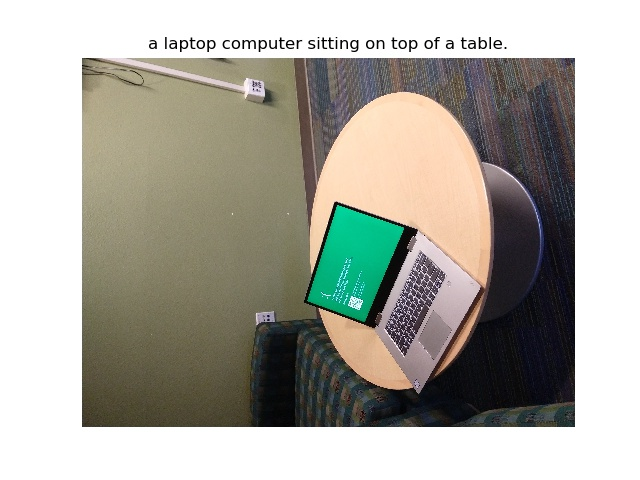
\includegraphics[width=0.75\textwidth]{assets/eg/r7_out.jpg}
\end{figure}
% subsection ends 
%----------------

\subsection{Conclusion}
It is clear from these experiments that, as the size of the available datasets for image description increases, so will the performance of approaches like NIC. However there are many scenarios on which the current model shows errors like the one here.
\begin{figure}[h!]
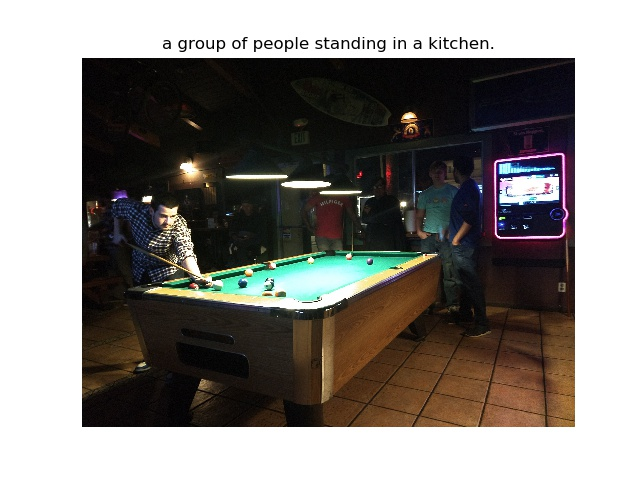
\includegraphics[width=0.75\textwidth]{assets/eg/err1_out.jpg}
\end{figure}
% subsection ends 
%----------------

%----------------------------------------------------------------------------------------

% section ends 
\LaTeX\
\end{document} to your LaTeX file where you want your
% title page.
%
%%%%%%%%%%%%%%%%%%%%%%%%%%%%%%%%%%%%%%%%%
%\title{Title page with logo}
%----------------------------------------------------------------------------------------
%	PACKAGES AND OTHER DOCUMENT CONFIGURATIONS
%----------------------------------------------------------------------------------------

\documentclass[12pt]{article}
\usepackage[english]{babel}
\usepackage[utf8x]{inputenc}
\usepackage{amsmath}
\usepackage{graphicx}
\usepackage[colorinlistoftodos]{todonotes}

\begin{document}

\begin{titlepage}

\newcommand{\HRule}{\rule{\linewidth}{0.5mm}} % Defines a new command for the horizontal lines, change thickness here

\center % Center everything on the page
 
%----------------------------------------------------------------------------------------
%	HEADING SECTIONS
%----------------------------------------------------------------------------------------

\textsc{\LARGE University of California, Santa Barbara}\\[1cm] % Name of your university/college
\textsc{\Large Project Report}\\[0.5cm] % Major heading such as course name

%----------------------------------------------------------------------------------------
%	TITLE SECTION
%----------------------------------------------------------------------------------------

\HRule \\[0.4cm]
{ \huge \bfseries Image Captioning}\\[0.1cm] % Title of your document
\HRule \\[1cm]
 
%----------------------------------------------------------------------------------------
%	AUTHOR SECTION
%----------------------------------------------------------------------------------------

\begin{minipage}{0.4\textwidth}
\begin{flushleft} \large
\emph{Author:}\\
Nikhil \textsc{S M} \\
Rahul \textsc{V} % Your name
\end{flushleft}
\end{minipage}
~
\begin{minipage}{0.4\textwidth}
\begin{flushright} \large
\emph{Supervisor:} \\
Prof Y F \textsc{Wang} % Supervisor's Name
\end{flushright}
\end{minipage}\\[2cm]

% If you don't want a supervisor, uncomment the two lines below and remove the section above
%\Large \emph{Author:}\\
%John \textsc{Smith}\\[3cm] % Your name

%----------------------------------------------------------------------------------------
%	DATE SECTION
%----------------------------------------------------------------------------------------

{\large \today}\\[1cm] % Date, change the \today to a set date if you want to be precise

%----------------------------------------------------------------------------------------
%	LOGO SECTION
%----------------------------------------------------------------------------------------


\includegraphics{assets/ucsb-logo.png}\\[1cm] % Include a department/university logo - this will require the graphicx package
 
%----------------------------------------------------------------------------------------
\vfill % Fill the rest of the page with whitespace
\end{titlepage}

%\begin{abstract}
%\end{abstract}

%----------------------------------------------------------------------------------------
\section{Objective}
Understand the Image Captioning problem in Computer vision and Natural language processing. Demonstrate components, process, training ( with batching, validation) and estimate performance (e.g., error rate vs. run time and iterations, resource usage statistics)
% section ends 

%----------------------------------------------------------------------------------------
\section{Introduction}
Automatically describing the contents of an image is a fundamental problem in computer vision and natural language processing. In this project we look at a generative model based on a deep recurrent architecture. The model is trained to maximize the likelihood of the target description sentence given the training image. Experiments on COCO image/text datasets show the accuracy of the model and the fluency of the language it learns solely from image descriptions.

This project based its implementation on the method described in the CVPR2015 paper "Show and Tell: A Neural Image Caption Generator". 
% section ends 

%----------------------------------------------------------------------------------------
\section{Model}
Model is based end-to-end on a neural network consisting of a vision CNN followed by a language generating RNN. The author's describe this model as Neural Image Caption or NIC.
% Include a shownntell figure here:
\begin{figure}[ht!]
\centering
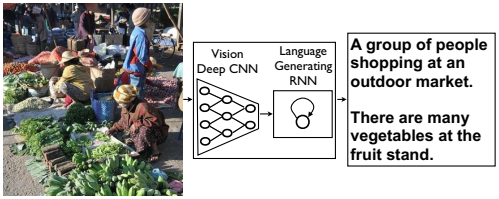
\includegraphics[width=0.8\textwidth]{assets/shownntell.png}
\caption{\label{fig:shownntell}NIC model (vision CNN followed by language generating RNN)}
\end{figure}

An “encoder” CNN reads the input images by embedding it to a fixed-length vector and transforms it into a rich fixed-length vector representation, which is pre-trained for an image classification task and using the last hidden layer as the initial hidden state of a “decoder” RNN that generates the target sentence. The RNN model uses a Long-Short Term Memory (LSTM) net, which has shown state-of-the art performance on sequence tasks such as translation.

% Include a model figure here:
\begin{figure}[ht!]
\centering
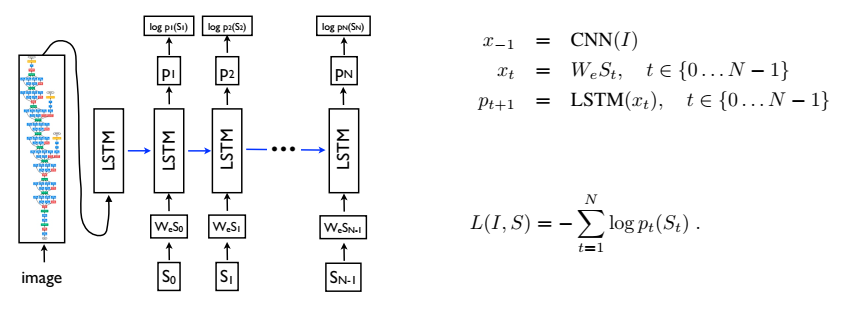
\includegraphics[width=1\textwidth]{assets/model.png}
\caption{\label{fig:model}LSTM model combined with a CNN image embedder. L(I,S) is the loss function with each word as a one-hot vector S\textsubscript{t}}.
\end{figure}

Both the image and the words are mapped to the same space, the image by using a vision CNN, the words by using word embedding W\textsubscript{e}. Inference is done by BeamSearch, keeping k best sentences up to time t as candidates to generate sentences of size t+1 and taking the resulting best.
% section ends 

%----------------------------------------------------------------------------------------
\section{Results}
\label{sec:results}

\subsection{Training}
The MS COCO dataset consists of JPEG images and text captions for each image.



Here is a brief on the training data configuration
% Describe the dataset
\begin{table}[ht!]
\centering
  \begin{tabular}{l|l|l|l}
    Dataset & training & valid & test  \\\hline
    MSCOCO & 82783 & 40504 & 40775\\
  \end{tabular}
\caption{\label{tab:dataset} MSCOCO Dataset}
\label{tab:dataset}
\end{table}

\begin{description}
  \item[$\bullet$ ] Initialized weights of CNN component to a pre-trained model (ImageNet).
  \item[$\bullet$ ] Preprocessing of MS-Coco Data set
  	\begin{description}
    	\item[$\cdot$ ] Creating a correspondence between image and the caption.
    \end{description}
  \item[$\bullet$ ] Creating a Word Embedding Matrix.
  \item[$\bullet$ ] Cross Entropy as Loss function
  \item[$\bullet$ ] Adam Optimizer with initial learning rate of 0.0001
  \item[$\bullet$ ] Training: 
    \begin{description}
      	\item[$\cdot$ ] Data Set : MS COCO as per Table~\ref{tab:dataset}
      	\item[$\cdot$ ] All RNN inputs are left padded.
      	\item[$\cdot$ ] Words are Embedded into 512 dimension vector.
      	\item[$\cdot$ ] A Batch size of 32 is used to run for 5 epochs.
      	\item[$\cdot$ ] BLEU Score is used as an evaluation metric.
    \end{description}
  \item[$\cdot$ ] Data Set : MS COCO as per Table~\ref{tab:dataset}
  \item[$\ast$ ]
\end{description}

Lets take a look at the workflow for establishing the training data

Data Description
The COCO data has JPG images with text captions for each image in a JSON file. We use the "image\_id", "image\_file" and "caption" fields from the captions .... 


\todo[inline, color=green!40]{Describe the training parameters measure, accuracies \& convergence}



\subsection{Metrics}
Here are the various metrics for MS COCO dataset. 
\todo{Describe the metrics!}
% Describe the metrics
\begin{table}[h!]
\centering
\begin{tabular}{l|l|l|l|l}
Metric & BLEU-1 & BLEU-2 & BLEU-3 & BLEU-4  \\\hline
Value & 62.9\% & 43.6\% & 29.0\% & 19.3\% \\
\end{tabular}
\caption{\label{tab:metrics}Scores on Dataset --- described in Table~\ref{tab:dataset}.}
\end{table}
% subsection ends 
%----------------

\subsection{Output}
Here are some test outputs generated by the Image captioning system \dots

\subsubsection{Images from the internet }
\begin{figure}[ht!]
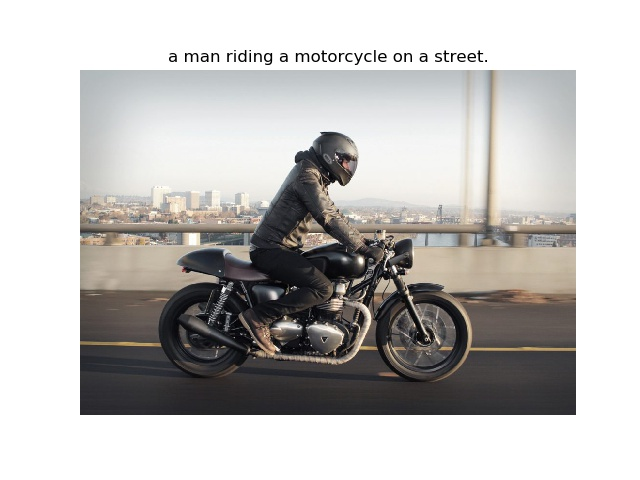
\includegraphics[width=0.75\textwidth]{assets/eg/r2_out.jpg}
\end{figure}
\begin{figure}[ht!]
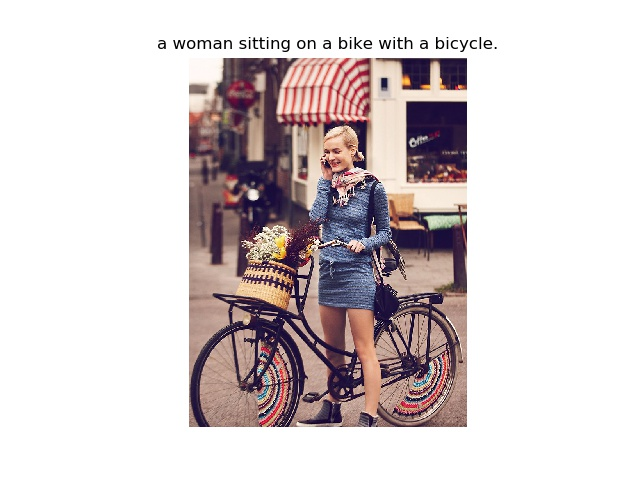
\includegraphics[width=0.75\textwidth]{assets/eg/r3_out.jpg}
\end{figure}
\begin{figure}[ht!]
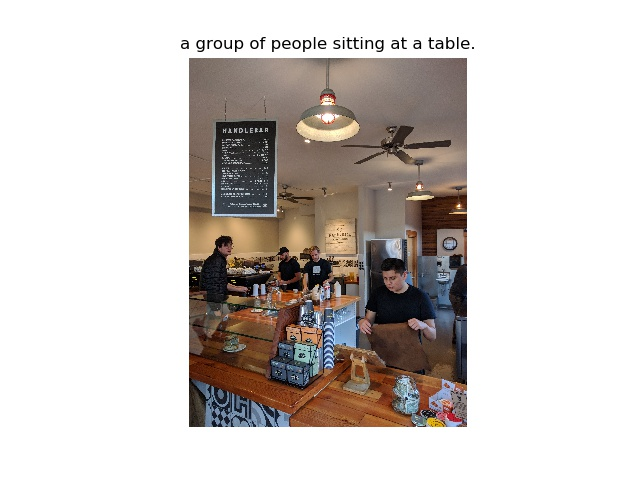
\includegraphics[width=0.75\textwidth]{assets/eg/r4_out.jpg}
\end{figure}

\subsubsection{Images from the Arrowhead common rooms}
\begin{figure}[ht!]
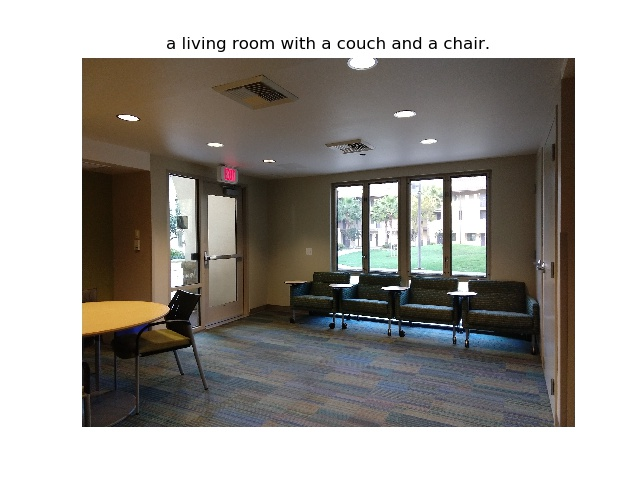
\includegraphics[width=0.75\textwidth]{assets/eg/r5_out.jpg}
\end{figure}
\begin{figure}[ht!]
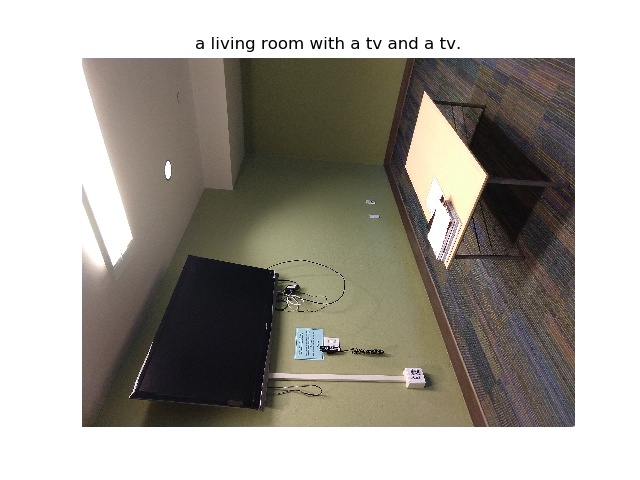
\includegraphics[width=0.75\textwidth]{assets/eg/r6_out.jpg}
\end{figure}
\begin{figure}[ht!]
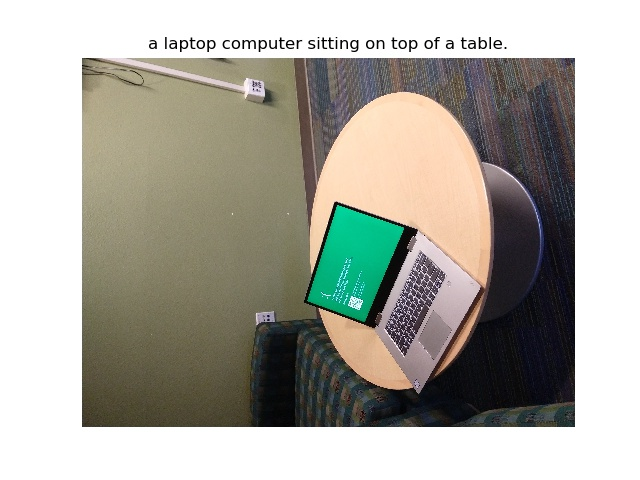
\includegraphics[width=0.75\textwidth]{assets/eg/r7_out.jpg}
\end{figure}
% subsection ends 
%----------------

\subsection{Conclusion}
It is clear from these experiments that, as the size of the available datasets for image description increases, so will the performance of approaches like NIC. However there are many scenarios on which the current model shows errors like the one here.
\begin{figure}[h!]
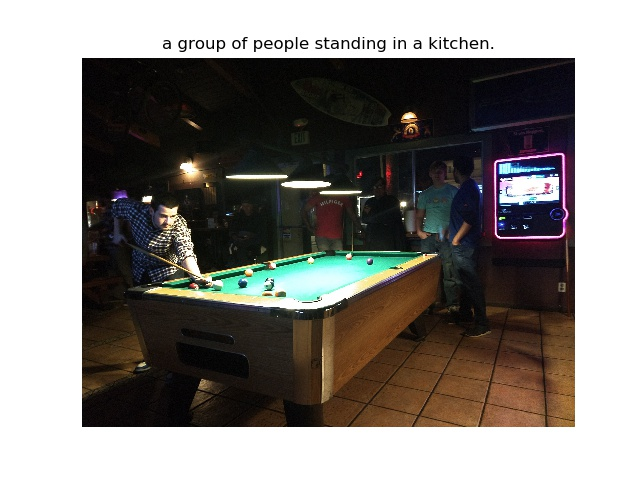
\includegraphics[width=0.75\textwidth]{assets/eg/err1_out.jpg}
\end{figure}
% subsection ends 
%----------------

%----------------------------------------------------------------------------------------

% section ends 
\LaTeX\
\end{document} to your LaTeX file where you want your
% title page.
%
%%%%%%%%%%%%%%%%%%%%%%%%%%%%%%%%%%%%%%%%%
%\title{Title page with logo}
%----------------------------------------------------------------------------------------
%	PACKAGES AND OTHER DOCUMENT CONFIGURATIONS
%----------------------------------------------------------------------------------------

\documentclass[12pt]{article}
\usepackage[english]{babel}
\usepackage[utf8x]{inputenc}
\usepackage{amsmath}
\usepackage{graphicx}
\usepackage[colorinlistoftodos]{todonotes}

\begin{document}

\begin{titlepage}

\newcommand{\HRule}{\rule{\linewidth}{0.5mm}} % Defines a new command for the horizontal lines, change thickness here

\center % Center everything on the page
 
%----------------------------------------------------------------------------------------
%	HEADING SECTIONS
%----------------------------------------------------------------------------------------

\textsc{\LARGE University of California, Santa Barbara}\\[1cm] % Name of your university/college
\textsc{\Large Project Report}\\[0.5cm] % Major heading such as course name

%----------------------------------------------------------------------------------------
%	TITLE SECTION
%----------------------------------------------------------------------------------------

\HRule \\[0.4cm]
{ \huge \bfseries Image Captioning}\\[0.1cm] % Title of your document
\HRule \\[1cm]
 
%----------------------------------------------------------------------------------------
%	AUTHOR SECTION
%----------------------------------------------------------------------------------------

\begin{minipage}{0.4\textwidth}
\begin{flushleft} \large
\emph{Author:}\\
Nikhil \textsc{S M} \\
Rahul \textsc{V} % Your name
\end{flushleft}
\end{minipage}
~
\begin{minipage}{0.4\textwidth}
\begin{flushright} \large
\emph{Supervisor:} \\
Prof Y F \textsc{Wang} % Supervisor's Name
\end{flushright}
\end{minipage}\\[2cm]

% If you don't want a supervisor, uncomment the two lines below and remove the section above
%\Large \emph{Author:}\\
%John \textsc{Smith}\\[3cm] % Your name

%----------------------------------------------------------------------------------------
%	DATE SECTION
%----------------------------------------------------------------------------------------

{\large \today}\\[1cm] % Date, change the \today to a set date if you want to be precise

%----------------------------------------------------------------------------------------
%	LOGO SECTION
%----------------------------------------------------------------------------------------


\includegraphics{assets/ucsb-logo.png}\\[1cm] % Include a department/university logo - this will require the graphicx package
 
%----------------------------------------------------------------------------------------
\vfill % Fill the rest of the page with whitespace
\end{titlepage}

%\begin{abstract}
%\end{abstract}

%----------------------------------------------------------------------------------------
\section{Objective}
Understand the Image Captioning problem in Computer vision and Natural language processing. Demonstrate components, process, training ( with batching, validation) and estimate performance (e.g., error rate vs. run time and iterations, resource usage statistics)
% section ends 

%----------------------------------------------------------------------------------------
\section{Introduction}
Automatically describing the contents of an image is a fundamental problem in computer vision and natural language processing. In this project we look at a generative model based on a deep recurrent architecture. The model is trained to maximize the likelihood of the target description sentence given the training image. Experiments on COCO image/text datasets show the accuracy of the model and the fluency of the language it learns solely from image descriptions.

This project based its implementation on the method described in the CVPR2015 paper "Show and Tell: A Neural Image Caption Generator". 
% section ends 

%----------------------------------------------------------------------------------------
\section{Model}
Model is based end-to-end on a neural network consisting of a vision CNN followed by a language generating RNN. The author's describe this model as Neural Image Caption or NIC.
% Include a shownntell figure here:
\begin{figure}[ht!]
\centering
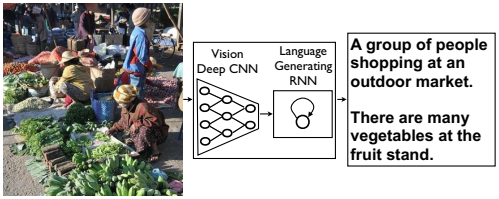
\includegraphics[width=0.8\textwidth]{assets/shownntell.png}
\caption{\label{fig:shownntell}NIC model (vision CNN followed by language generating RNN)}
\end{figure}

An “encoder” CNN reads the input images by embedding it to a fixed-length vector and transforms it into a rich fixed-length vector representation, which is pre-trained for an image classification task and using the last hidden layer as the initial hidden state of a “decoder” RNN that generates the target sentence. The RNN model uses a Long-Short Term Memory (LSTM) net, which has shown state-of-the art performance on sequence tasks such as translation.

% Include a model figure here:
\begin{figure}[ht!]
\centering
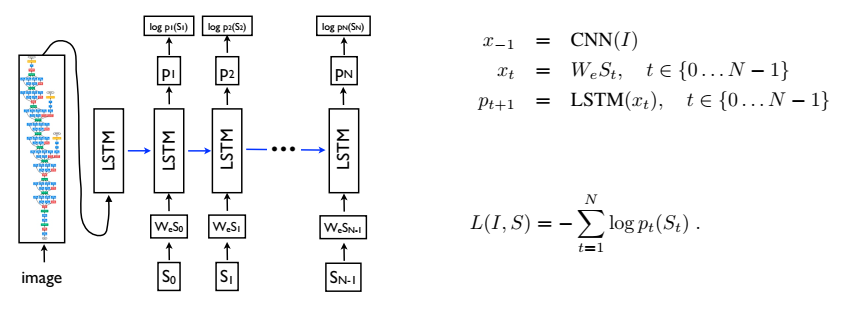
\includegraphics[width=1\textwidth]{assets/model.png}
\caption{\label{fig:model}LSTM model combined with a CNN image embedder. L(I,S) is the loss function with each word as a one-hot vector S\textsubscript{t}}.
\end{figure}

Both the image and the words are mapped to the same space, the image by using a vision CNN, the words by using word embedding W\textsubscript{e}. Inference is done by BeamSearch, keeping k best sentences up to time t as candidates to generate sentences of size t+1 and taking the resulting best.
% section ends 

%----------------------------------------------------------------------------------------
\section{Results}
\label{sec:results}

\subsection{Training}
The MS COCO dataset consists of JPEG images and text captions for each image.



Here is a brief on the training data configuration
% Describe the dataset
\begin{table}[ht!]
\centering
  \begin{tabular}{l|l|l|l}
    Dataset & training & valid & test  \\\hline
    MSCOCO & 82783 & 40504 & 40775\\
  \end{tabular}
\caption{\label{tab:dataset} MSCOCO Dataset}
\label{tab:dataset}
\end{table}

\begin{description}
  \item[$\bullet$ ] Initialized weights of CNN component to a pre-trained model (ImageNet).
  \item[$\bullet$ ] Preprocessing of MS-Coco Data set
  	\begin{description}
    	\item[$\cdot$ ] Creating a correspondence between image and the caption.
    \end{description}
  \item[$\bullet$ ] Creating a Word Embedding Matrix.
  \item[$\bullet$ ] Cross Entropy as Loss function
  \item[$\bullet$ ] Adam Optimizer with initial learning rate of 0.0001
  \item[$\bullet$ ] Training: 
    \begin{description}
      	\item[$\cdot$ ] Data Set : MS COCO as per Table~\ref{tab:dataset}
      	\item[$\cdot$ ] All RNN inputs are left padded.
      	\item[$\cdot$ ] Words are Embedded into 512 dimension vector.
      	\item[$\cdot$ ] A Batch size of 32 is used to run for 5 epochs.
      	\item[$\cdot$ ] BLEU Score is used as an evaluation metric.
    \end{description}
  \item[$\cdot$ ] Data Set : MS COCO as per Table~\ref{tab:dataset}
  \item[$\ast$ ]
\end{description}

Lets take a look at the workflow for establishing the training data

Data Description
The COCO data has JPG images with text captions for each image in a JSON file. We use the "image\_id", "image\_file" and "caption" fields from the captions .... 


\todo[inline, color=green!40]{Describe the training parameters measure, accuracies \& convergence}



\subsection{Metrics}
Here are the various metrics for MS COCO dataset. 
\todo{Describe the metrics!}
% Describe the metrics
\begin{table}[h!]
\centering
\begin{tabular}{l|l|l|l|l}
Metric & BLEU-1 & BLEU-2 & BLEU-3 & BLEU-4  \\\hline
Value & 62.9\% & 43.6\% & 29.0\% & 19.3\% \\
\end{tabular}
\caption{\label{tab:metrics}Scores on Dataset --- described in Table~\ref{tab:dataset}.}
\end{table}
% subsection ends 
%----------------

\subsection{Output}
Here are some test outputs generated by the Image captioning system \dots

\subsubsection{Images from the internet }
\begin{figure}[ht!]
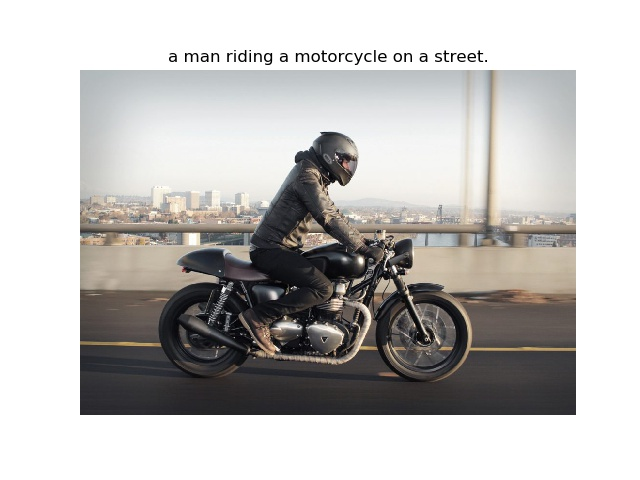
\includegraphics[width=0.75\textwidth]{assets/eg/r2_out.jpg}
\end{figure}
\begin{figure}[ht!]
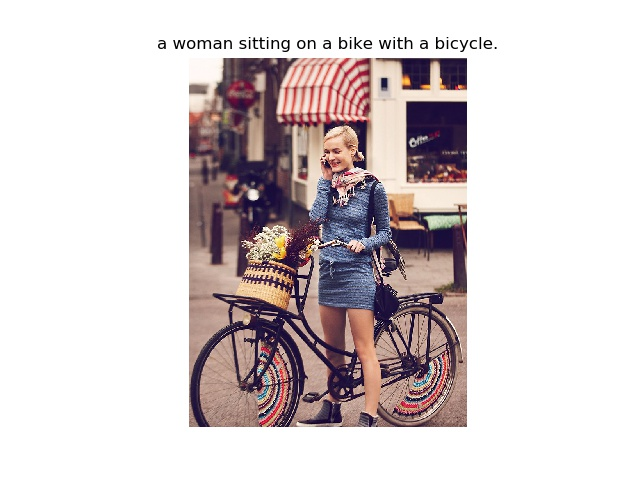
\includegraphics[width=0.75\textwidth]{assets/eg/r3_out.jpg}
\end{figure}
\begin{figure}[ht!]
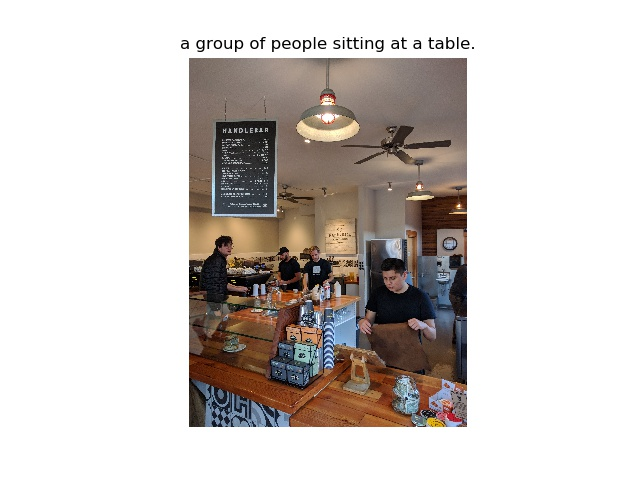
\includegraphics[width=0.75\textwidth]{assets/eg/r4_out.jpg}
\end{figure}

\subsubsection{Images from the Arrowhead common rooms}
\begin{figure}[ht!]
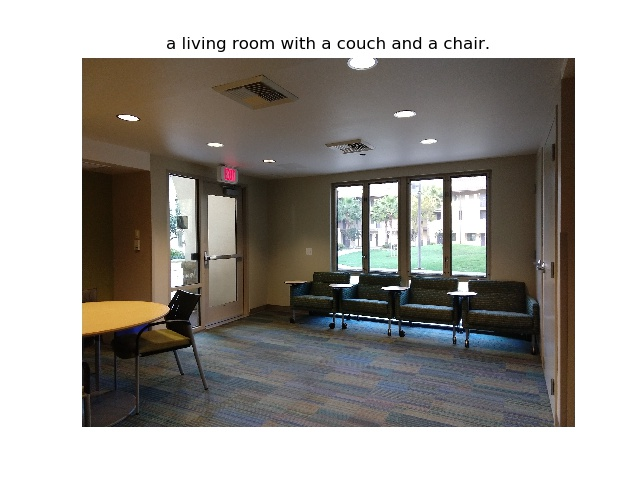
\includegraphics[width=0.75\textwidth]{assets/eg/r5_out.jpg}
\end{figure}
\begin{figure}[ht!]
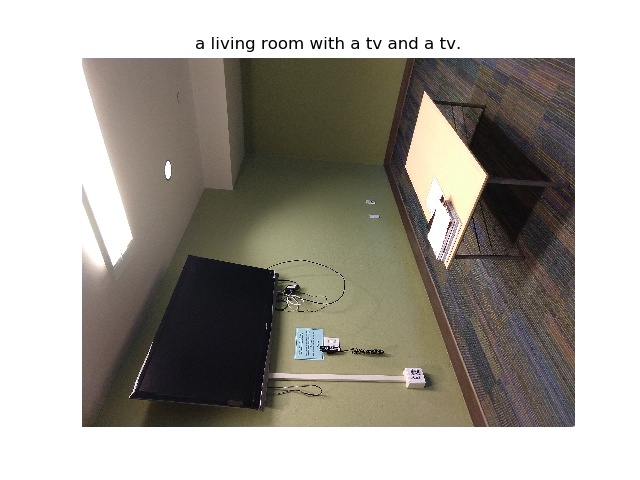
\includegraphics[width=0.75\textwidth]{assets/eg/r6_out.jpg}
\end{figure}
\begin{figure}[ht!]
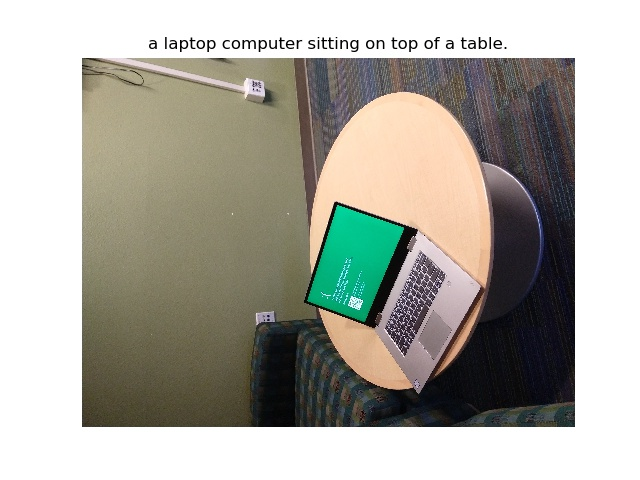
\includegraphics[width=0.75\textwidth]{assets/eg/r7_out.jpg}
\end{figure}
% subsection ends 
%----------------

\subsection{Conclusion}
It is clear from these experiments that, as the size of the available datasets for image description increases, so will the performance of approaches like NIC. However there are many scenarios on which the current model shows errors like the one here.
\begin{figure}[h!]
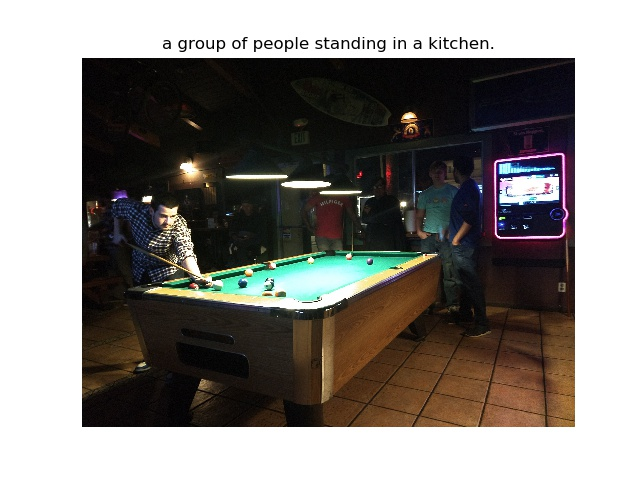
\includegraphics[width=0.75\textwidth]{assets/eg/err1_out.jpg}
\end{figure}
% subsection ends 
%----------------

%----------------------------------------------------------------------------------------

% section ends 
\LaTeX\
\end{document}